% !TEX program = xelatex
\documentclass[bwprint,fontset=fandol]{gmcmthesis}
\hypersetup{hidelinks}
\pdfstringdefDisableCommands{\def\kern#1{}}
\usepackage{siunitx}
\usepackage{booktabs}
\usepackage{graphicx}
\usepackage{tabularx}
\emergencystretch=3em
\title{山区洪涝灾害下无人机运输与通信协同优化}
\baominghao{\hspace{6em}26106350114}
\schoolname{\hspace{5.8em}西南大学}
\membera{\hspace{6em}谢文哲}
\memberb{\hspace{6em}章林怡}
\memberc{\hspace{6em}刘宇豪}

\begin{document}
\maketitle
\begin{abstract}
针对山区洪涝灾害中道路与通信同时受损的物资配送任务，本文使用题给服务区、货箱、异构无人机、能源设备和30\,m数字高程模型（DEM），依次求解单点安全载荷与组批、多机多架次运输、通信中继联合调度及固定任务分区。四问共用按地形确定的爬升--巡航--下降航段、载荷相关能耗、返航余量和分段充电模型。

问题一以二分法求45个机型--服务区组合的安全载荷，并以动态规划处理80个不可拆货箱，得到18个架次和59.131\,kWh运输能耗。问题二先生成物理可行的多点候选架次，再以CP-SAT选择路线、安排运输机与共享电池，并在固定路线后重排任务开始时刻。所得24个运输架次唯一交付全部80箱，其中2个架次跨服务区；加权迟到为0，运输能耗69.580\,kWh，完工时间6997.523\,s。固定这24条路线后的整数秒资源排程有最优性证书，但全路线空间没有全局最优证明。

问题三在题给DEM和双向链路预算下建立运输机直连网关或由中继两跳保障的全时段约束。有限宽度搜索与经验证的时间窗口细化得到24个运输架次、5个中继架次，联合完工时间8772.339\,s，总能耗73.835\,kWh，加权迟到8546.904优先系数秒；80箱唯一交付，硬时限、资源冲突和通信中断均为0。逐秒回代和覆盖全部36198.242\,s运输作业时间的连续通信证书均通过。问题四在固定第三问任务与保障关系下枚举分区，两组、三组独立执行分别至少存在2、4项现有库存缺口。本文的运输与中继方案属于已验证的可行启发式解。
\keywords{山区应急运输\quad 异构无人机\quad 多架次调度\quad 通信中继\quad 连续时间验证}
\end{abstract}

\pagestyle{plain}
\maketoc
\clearpage
\section{问题重述与数据}
题目要求解决四个递进任务：单点往返运输能力和货箱组批；允许跨服务区访问时的路线与设备周转；加入山区遮挡及通信中继，保证运输全过程通信；在第三问任务固定时将服务区分为两个或三个独立执行组。基础数据包含调度中心$O_{01}$、15个服务区、80个不可拆货箱、A/B/C三型共8架运输机、2架中继机、共享电池、6个中继能源组件和30\,m DEM~\cite{problem}。时刻均以题目任务起点为零点，电能单位为kWh。

由DEM像元求每条直飞航段的最高地面高程，再生成候选架次及交付偏移量。问题二的排程成为问题三的初始运输方案；问题四只读取问题三已经确定的任务与保障关系。四问使用同一物理参数回代，计算链条见图~\ref{fig:overall-flow}。
\begin{figure}[htbp]
\centering

\includegraphics[width=0.94\textwidth]{figures/flow_overall_model.pdf}
\caption{四个问题从基础数据、运输物理模型到排程、通信验证及分区配置的衔接}
\label{fig:overall-flow}
\end{figure}

\section{统一假设与物理模型}
\subsection{符号与边界}
记货箱、候选运输架次、运输机型集合为$\mathcal B,\mathcal P,\mathcal G$。箱$b$的质量、体积、优先系数、期望时刻和硬截止时刻分别为$m_b,v_b,w_b,D_b,H_b$；架次$p$的任务开始（准备开始）时刻、箱$b$的交付偏移和返航时刻为$s_p,\delta_{pb},F_p$。第二、三问反复使用的符号列于表~\ref{tab:symbols-q23}。每箱不可拆且只交付一次，每个运输架次均从$O_{01}$出发并返回。到服务区交接完成后，才扣除对应货箱质量。题面未分别展开水平能耗和爬升能耗，本文以等效航程换算水平电耗，并以重力势能除以效率计入爬升电耗；下降不另计附加电耗。题面未限定单架中继的并发接入数，故按可共享覆盖点处理。
\begin{table}[htbp]
\centering\small
\caption{第二、三问主要符号}
\label{tab:symbols-q23}
\begin{tabularx}{0.95\textwidth}{@{}lXl@{}}
\toprule
符号 & 含义 & 单位\\
\midrule
$\mathcal P,\ B_p$ & 候选运输架次集合、候选$p$承运的货箱集合 & ---\\
$s_p,\ d_p,\ \delta_{pb}$ & 架次准备开始时刻、作业时长、货箱交付偏移 & s\\
$C_b,\ D_b,\ H_b$ & 交付时刻、期望时刻、硬截止时刻 & s\\
$E_p,\ \rho_g$ & 运输架次能耗、机型返航电量比例下限 & kWh，1\\
$N_g^{\rm drone},N_g^{\rm bat}$ & 同型运输机和共享电池库存 & 架，块\\
$L^{\max}_{a\leftrightarrow b},L_{ab}(t)$ & 双向允许路径损耗、实际路径损耗 & dB\\
$A_{ab}(t), I_r(t)$ & 链路可用指示量、中继服务指示量 & 0或1\\
$[\sigma_r,\tau_r]$ & 中继$r$建链后的服务窗口 & s\\
$E_r^{\rm relay}$ & 一次中继架次的总电耗 & kWh\\
\bottomrule
\end{tabularx}
\end{table}

\subsection{航段时间、能耗和充电}
机型$g$在载重$q$时的等效航程按题给关系计算：
\begin{equation}
L_g(q)=L_g(0)-[L_g(0)-L_g(Q_g)](q/Q_g)^{3/2}.
\end{equation}
直飞航段$i\to j$的巡航海拔为经过DEM像元的最高地面高程加50\,m。中心作业高度取地面，服务区取地面加30\,m。令$d_{ij}$为水平距离，$h_{ij}^{+},h_{ij}^{-}$为爬升、下降量，则
\begin{align}
t_{gij}&=h_{ij}^{+}/v_g^{\uparrow}+d_{ij}/v_g^c+h_{ij}^{-}/v_g^{\downarrow},\\
e_{gij}(q)&=E_g^{\rm use}d_{ij}/L_g(q)
+9.81(m_g^0+q)h_{ij}^{+}/(3.6\times10^6\eta_g).
\end{align}
$E_g^{\rm use}$为额定可用电能，$m_g^0$为空机质量，$\eta_g$为爬升效率。各航段电耗求和为$E_p$，须满足$E_p\le(1-\rho_g)E_g^{\rm use}$，并满足机型载重、体积上限。架次还计入准备、逐箱装载与服务区卸载。箱$b$在交接结束时送达，故$C_b=s_p+\delta_{pb}$。

返航电量比例$u_p=1-E_p/E_g^{\rm use}$。若$T_g^{\rm full}$为题给完全充电时间，则
\begin{equation}
T_g^{\rm chg}(u)=
\begin{cases}
T_g^{\rm full}[0.65(0.90-u)/0.90+0.35],&u<0.90,\\
0.35T_g^{\rm full}(1-u)/0.10,&u\geq0.90.
\end{cases}
\label{eq:charge}
\end{equation}
同一实体机在返航前、同一共享电池在充满前均不能再次投入任务。

\section{问题一：单点安全载荷与组批}
对于机型$g$和服务区$a$，单点往返安全载荷为
\begin{equation}
q_{ga}^{\max}=\max\{0\leq q\leq Q_g:
e_{g,O_{01}a}(q)+e_{g,aO_{01}}(0)\leq(1-\rho_g)E_g^{\rm use}\}.
\end{equation}
能耗随载荷单调不减，故在额定载荷不可行时二分求阈值。再按各区物资类别箱数向量$s$枚举满足质量、体积和能量约束的批次$k$及机型$g$，令
\begin{equation}
\mathbf F_a(s)=\mathop{\mathrm{lexmin}}_{g,\;0<k\leq s}
\{\mathbf F_a(s-k)+(1,e_a(g,k),t_a(g,k))\},
\end{equation}
依次比较架次数、总电耗、累计作业时间。逐区回溯后得到18架次，总能耗为59.131\,kWh，累计作业时间为32776.016\,s。逐箱回代无违规。在给定数据下，把返航余量提高至30\%使最少架次增至20；提高至40\%时现有机型不能完成全部货箱。

\section{问题二的建模与求解}
\subsection{问题二分析}
问题一把各服务区分开组批，因而未涉及实体无人机和电池在时间上的竞争。问题二允许同一架次访问多个服务区；一条路线的箱数、访问顺序和机型一经改变，沿途载荷、送达时刻及返航电量都会随之变化。即使若干架次分别满足航程约束，同时起飞也可能超过同型运输机或共享电池的库存。因此，本问须同时决定“哪些架次执行”和“何时由哪套设备执行”。

本文把单架次的空间与物理计算放在候选路线预处理中，把货箱覆盖、时限和资源周转放在整数排程中处理。前者保留多点访问的可能性，后者使运输机与电池的占用时段能够统一比较。图~\ref{fig:q2-resources}展示最终方案的两类资源时间轴；其中浅色区间是电池返航后充电及保守预留时间，不能作为下一架次的可用时间。

\subsection{基本约定与候选架次构造}
记$\mathcal B$为80个不可拆货箱集合，$\mathcal P$为预处理得到的候选运输架次。一个候选$p$包含货箱集合$B_p$、机型$g_p$和有序服务区序列$(a_1,\ldots,a_k)$，其路径为$O_{01}\to a_1\to\cdots\to a_k\to O_{01}$。同一服务区的货箱在一次停靠中交接；每个架次从满电池出发，到中心返航后才可更换或复用资源。货箱交付时刻取对应服务区卸载和交接结束时刻。

\subsubsection{逐航段载荷、时间和能源}

设$p$在航段$j$开始前尚未交付的货箱质量为$q_{pj}$，则
$q_{p1}=\sum_{b\in B_p}m_b$，每到达一个服务区后，扣除该服务区在本架次中已经交付的货箱质量。

设架次$p$中第$j$个航段的起点和终点分别为$u_j$和$v_j$。沿用问题一建立的航段飞行时间模型$t_{ij}(g)$和航段能耗模型$E_{ij}(g\mid q)$，则架次$p$的总作业时间和总能耗分别为

\begin{equation}
\begin{aligned}
d_p={}&t^{\rm prep}_{g_p}+|B_p|t^{\rm load}_{g_p}
+\sum_{j\in p}t_{u_jv_j}(g_p)\\
&+\sum_{a\in p}
\left(
t^{\rm service}_{g_p}
+|B_p\cap B_a|t^{\rm unload}_{g_p}
\right),
\\
E_p={}&\sum_{j\in p}E_{u_jv_j}(g_p\mid q_{pj}).
\end{aligned}
\label{eq:q2-route-physics}
\end{equation}

交付偏移$\delta_{pb}$按同一时间线累计到箱$b$完成交接为止。候选架次只有在起飞质量、体积、逐段航迹以及
\[
E_p\le(1-p_{g_p})E_{g_p}
\]
均满足要求时才予以保留；即使立即开始准备也无法满足硬时限的候选同样剔除。这样能够延续问题一的载荷相关能耗计算方法，并准确反映跨区架次在首站卸货后载荷下降对后续航段能耗的影响。
候选池先纳入问题一的单区组批、单箱和同区双箱方案，再用固定随机种子的受限组批构造更多组合，至多访问三个服务区，并对同一货箱组合尝试其他可行机型。相同“机型—货箱集合—访问顺序”去重后，排程器面对3988条有限候选路线。这个规模是计算设计，不代表全部可能路线均已穷举。

\subsection{货箱覆盖、时限与共享资源模型}
\subsubsection{一次交付和时限}
令$x_p\in\{0,1\}$表示是否执行候选$p$，$s_p\in\mathbb Z_{\geq0}$为其准备开始时刻。任何货箱恰由一条选中路线交付：
\begin{equation}
\sum_{p:\,b\in B_p}x_p=1,\qquad b\in\mathcal B.
\label{eq:q2-cover}
\end{equation}
箱$b$在被选中的架次$p$中完成交接的实际时刻为$C_b=s_p+\delta_{pb}$。对具有硬截止时刻$H_b$的首批保障箱及医疗箱施加$C_b\le H_b$；题给期望时刻$D_b$用于衡量迟到，令$T_b=\max\{0,C_b-D_b\}$。当同一箱同时受到首批保障和医疗时限约束时，取较早的硬截止时刻。未设置硬截止的箱可以迟于$D_b$，但会付出加权迟到代价。

\subsubsection{运输机与共享电池的双区间占用}
记机型$g$现有运输机数和电池数为$N_g^{\rm drone},N_g^{\rm bat}$，本题分别为A型$4/6$、B型$2/4$、C型$2/4$。运输机占用到实际返航，电池则还须经历式~\eqref{eq:charge}给出的分段充电。为在整数秒排程中保守处理非整数时长，定义
\begin{equation}
\widehat d_p=\lceil d_p\rceil,\qquad
\widehat b_p=\left\lceil d_p+T_{g_p}^{\rm chg}
\left(1-\frac{E_p}{E_{g_p}^{\rm use}}\right)\right\rceil.
\label{eq:q2-reserved-length}
\end{equation}
选择架次$p$时，运输机占用$[s_p,s_p+\widehat d_p)$，电池占用$[s_p,s_p+\widehat b_p)$。对每种机型和任意时刻$t$，两类并发数分别不得超过其库存：
\begin{align}
\sum_{p:g_p=g}x_p\mathbf 1_{[s_p,s_p+\widehat d_p)}(t)
&\le N_g^{\rm drone},\\
\sum_{p:g_p=g}x_p\mathbf 1_{[s_p,s_p+\widehat b_p)}(t)
&\le N_g^{\rm bat}.
\label{eq:q2-cumulative}
\end{align}
整数模型中两组区间分别用可选区间与累积容量约束表达。求解后再按区间不重叠原则把任务匹配至具体机号、电池号，并以未取整的物理时刻复核。此时表~\ref{tab:q2-result}中的完工时间按实际返航计算，与整数目标中的向上取整完工值略有差别。

\subsection{优化目标与求解方法}
\subsubsection{整数化加权目标}
本问同时关心送达及时性、最后返航时间、能耗和架次数。为使求解器能够直接比较不同候选路线，采用代码中\texttt{balanced}配置的单一整数目标。设$\widehat C_b=s_p+\lceil\delta_{pb}\rceil$、$\widehat T_b=\max(0,\widehat C_b-D_b)$，并令$\widehat M=\max_{p:x_p=1}(s_p+\widehat d_p)$，则
\begin{equation}
\min\;100\widehat M
+\sum_{b\in\mathcal B}w_b\bigl(\widehat C_b+100\widehat T_b\bigr)
+\sum_{p\in\mathcal P}x_p\left[10\,\operatorname{round}(1000E_p)+10000\right].
\label{eq:q2-objective}
\end{equation}
这里$w_b$是题给优先系数。式~\eqref{eq:q2-objective}是加权和，并非严格字典序；报告“迟到为零”是求得排程的事实，不应理解为目标函数强制零迟到。能耗项以Wh取整，所有系数均为本次计算采用的权重，不把它们解释成真实货币成本。

\subsubsection{候选池求解与固定路线重排}
CP-SAT先在有限候选池内联合选择路线和任务开始时刻，原始排程目标值为4290638。随后固定24条选中路线和货箱分配，只重排整数秒开始时刻及两类容量资源。新目标值为4281382，较原排程减少9256（约0.216\%）。此固定路线子问题的求解状态为\texttt{OPTIMAL}，目标值与下界同为4281382。

为考察更换组批和访问顺序的可能改进，还进行了20轮大邻域重建：每轮移出5--9条当前路线，补入相关替代路线和部分成对合并路线，给CP-SAT 8\,s搜索时间，随机种子为20260923。20轮均未接受更优解；因此，本次已实现的目标值改善来自前述\emph{固定路线重排}，不能归因于大邻域搜索。“固定路线最优”也仅针对这24条路线、整数秒开始时刻和给定资源模型，不证明3988条候选池或全部可行路线上的全局最优。

\subsection{计算结果与分析}
\subsubsection{运输任务与机型分工}
表~\ref{tab:q2-result}给出正式方案。24个架次交付80箱，A、B、C型分别执行10、8、6架次；其中C型6架次承运39箱，体现大载重机型的组批能力。仅两条架次访问两个服务区：\texttt{Q2-009}沿$S009\to S012$运行，\texttt{Q2-020}沿$S011\to S014$运行。跨区比例较小，说明在给定地形、时限和能源条件下，多点访问并非对每批货箱都合算。

\begin{table}[htbp]
\centering\small
\caption{问题二正式运输方案的汇总结果}
\label{tab:q2-result}
\begin{tabular}{@{}lrrr@{}}
\toprule
指标 & A型 & B型 & C型\\
\midrule
运输架次 & 10 & 8 & 6\\
交付货箱数 & 20 & 21 & 39\\
运输能耗/kWh & 27.125 & 17.716 & 24.740\\
\midrule
\multicolumn{3}{@{}l}{全部货箱/全部架次} & 80 / 24\\
\multicolumn{3}{@{}l}{加权迟到/迟到箱数} & 0 / 0\\
\multicolumn{3}{@{}l}{运输返航完工时间/s} & 6997.523\\
\multicolumn{3}{@{}l}{总运输能耗/kWh} & 69.580\\
\multicolumn{3}{@{}l}{最小返航电量比例} & 23.088\%\\
\multicolumn{3}{@{}l}{最小硬时限剩余时间/s} & 220.525\\
\bottomrule
\end{tabular}
\end{table}

图~\ref{fig:q2-resources}按具体机号和电池号绘制排程。前8个架次在任务起点同时开始准备，之后的任务由已返航运输机及可用电池接续执行。若只看运输机的空闲而忽略下方浅色充电区间，就会高估可同时出动的能力；本图也给出了同型电池在不同实体机之间周转的实际安排。
\begin{figure}[htbp]
\centering
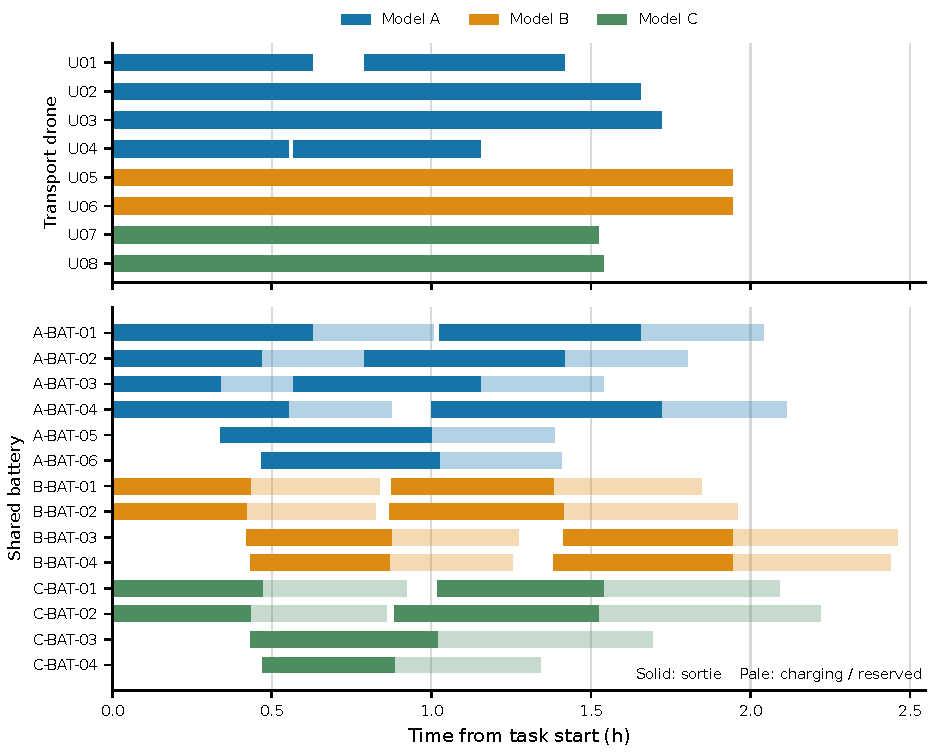
\includegraphics[width=0.96\textwidth]{figures/result_q2_resources.pdf}
\caption{问题二正式方案的运输机与共享电池占用时间轴；浅色部分为返航后的电池充电和保守预留区间}
\label{fig:q2-resources}
\end{figure}

\subsubsection{送达时效与安全余量}
80箱均在期望时刻前交付，加权迟到为零；按优先系数加权的平均交付时刻为2766.981\,s。具有硬截止时刻的货箱在图~\ref{fig:q2-slack}中均位于零线右侧。最紧的是饮用水箱\texttt{S012-\allowbreak{}WAT-01}，仍提前220.525\,s。若临时延迟相关架次，应首先复查此箱的硬时限。所有架次最小返航电量比例为23.088\%。
\begin{figure}[htbp]
\centering
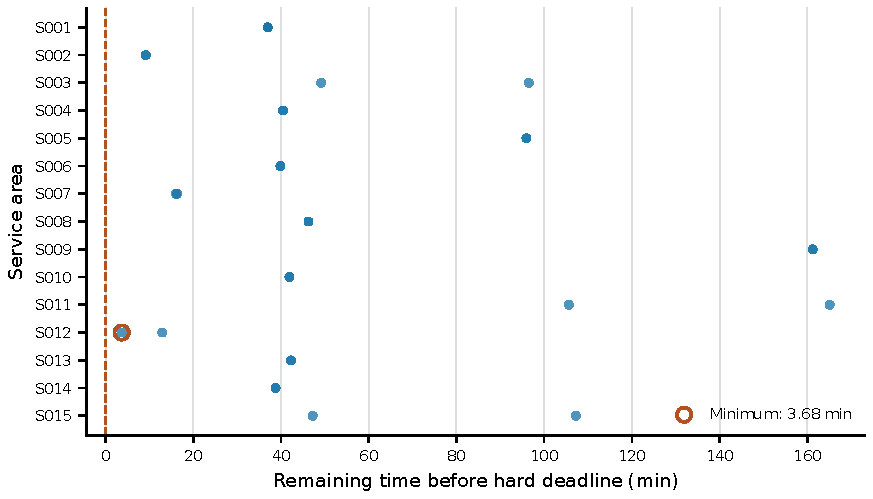
\includegraphics[width=0.86\textwidth]{figures/result_q2_hard_deadline_margin.pdf}
\caption{问题二各服务区有限硬时限货箱的送达余量；圈示最紧的\texttt{S012-WAT-01}}
\label{fig:q2-slack}
\end{figure}

\subsection{正确性与最优性范围检验}
由正式逐箱交付表检查，80个货箱各出现一次且无重复、漏投；由逐航段记录重新累加航时与能耗，并核对质量、体积及返航电量；由具体机号和电池号检查任务区间、充电区间不重叠。逐箱硬时限违反数和资源冲突数均为零。固定路线CP-SAT证书给出目标值与下界相等，证明的是这组路线的整数秒排程最优；整数时间模型采用向上取整的资源区间，正式物理结果再以连续实数时刻回代。候选池有限且大邻域搜索未取得新解，故完整第二问仍作为已验证可行方案报告。第三问将在此运输方案的基础上加入连续通信约束，并允许为保障通信重新安排部分运输时刻。

\section{问题三的建模与求解}
\subsection{问题三分析}
问题二的24架次排程满足运输与电池周转约束，却没有检查飞行过程中能否持续与固定网关$G_{01}$通信。山区遮挡使“起飞点、服务区两端可连通”不能推出整条航迹可连通；中继又占用两架中继机和六个能源组件，其建链、悬停及充电会反过来限制运输任务开始时刻。本问因而在已有货箱分配的基础上联动调整运输时序、中继位置和服务窗口，要求每一条运输轨迹的全部需通信时段都存在有效双向链路。

初始第二问排程的直连失效比例在不同架次间差异明显，见图~\ref{fig:q3-direct-gap}。图中比例是预计算网格上的诊断量，并非最终连续通信证明。中继位置若只为一个架次选择，可能产生大量短窗口；若能覆盖多条轨迹，就有机会减少中继起降和组件占用。因此，求解中把覆盖能力与任务时序同时考虑。
\begin{figure}[htbp]
\centering

\includegraphics[width=0.82\textwidth]{figures/raw_q3_q2_direct_outages.pdf}
\caption{问题二初始运输架次的网格化直连失效比例；通信约束尚未施加}
\label{fig:q3-direct-gap}
\end{figure}

\subsection{通信链路与连续覆盖模型}
\subsubsection{双向链路预算}
对端点$a,b$，由发射功率、收发增益、系统损耗和接收灵敏度计算两个方向的允许路径损耗，并取较小值作为双向门槛。若题给8\,dB通信裕量已计入接收门槛$P_{{\rm th},a}$、$P_{{\rm th},b}$，则
\begin{equation}
L^{\max}_{a\leftrightarrow b}
=\min\!\left\{
P_a+G_a^t+G_b^r-L_{\rm sys}-P_{{\rm th},b},\;
P_b+G_b^t+G_a^r-L_{\rm sys}-P_{{\rm th},a}
\right\}.
\label{eq:q3-budget}
\end{equation}
式中发射功率与接收门槛以dBm计，天线增益以dBi计，系统损耗与路径损耗以dB计。给定时刻$t$两端点三维距离$D_{ab}(t)$（km）、工作频率$f$（MHz），用DEM判定视线是否被地形遮挡，记遮挡指示量为$z_{ab}(t)$，则
\begin{equation}
L_{ab}(t)=32.45+20\log_{10}f+20\log_{10}D_{ab}(t)
+L_{\rm obs}z_{ab}(t),\qquad
A_{ab}(t)=\mathbf1\!\left\{L_{ab}(t)\le L^{\max}_{a\leftrightarrow b}\right\}.
\label{eq:q3-link}
\end{equation}
这里$L_{\rm obs}$是题给遮挡附加损耗。运输机位置按准备后爬升、水平巡航、下降和服务区交接阶段分段计算，而非把整条路线视为一根静态直线。

\subsubsection{直连或单中继两跳保障}
记运输机$p$的通信需求时间集合为$\mathcal T_p$。若中继任务$r$已完成建链并处于悬停服务窗口，令$I_r(t)=1$；否则为0。对所有$p$及$t\in\mathcal T_p$，要求
\begin{equation}
A_{pG}(t)=1
\quad\text{或}\quad
\exists r:\ I_r(t)A_{pr}(t)A_{rG}(t)=1.
\label{eq:q3-cover}
\end{equation}
因此，两跳链路必须在\emph{同一时刻}同时成立，不能分别用不同时刻的可达性代替。模型只使用固定网关直连或“运输机—中继—网关”两跳，不引入多中继转发。题目没有给出单架中继的并发接入上限；在这一数据边界下，同一中继服务窗可同时保障多架运输机。

\subsection{中继任务与能源资源模型}
\subsubsection{候选悬停点与预筛}
候选点以服务区、中心至服务区航线上的四分点和中点及服务区附近点为基础，并在部分位置枚举不同离地高度。每个位置均由DEM取得地面高程，悬停高度不超过题给上限。候选点需同时满足中继至网关的双向回传链路、往返飞行能量和返航余量。对每条运输轨迹上的直连缺口，预计算可由哪些候选点接入；图~\ref{fig:q3-sites}列出覆盖初始失联采样较多的一组候选点，说明位置选择直接影响后续可合并的服务窗口数量。该图用于筛选和解释搜索，不作为最终连续可行性的证据。
\begin{figure}[htbp]
\centering

\includegraphics[width=0.82\textwidth]{figures/process_q3_candidate_coverage.pdf}
\caption{候选中继点对初始运输轨迹直连失效采样点的覆盖数量；每个候选点独立统计}
\label{fig:q3-sites}
\end{figure}

\subsubsection{一次中继架次的时间与电量}
一条中继架次从$O_{01}$起飞，经历准备、往程、建链、悬停服务、返程和周转。设候选点为$k_r$，建链后服务窗口为$[\sigma_r,\tau_r]$，则其电耗写为
\begin{equation}
E_r^{\rm relay}=E_r^{\rm flight}
+\frac{P_{\rm hover}+P_{\rm comm}}{3600}
\bigl(T_{\rm link}+\tau_r-\sigma_r\bigr).
\label{eq:q3-relay-energy}
\end{equation}
$E_r^{\rm flight}$由往返水平飞行功率和爬升势能共同计算；$P_{\rm hover},P_{\rm comm}$以kW计，式中时间以s计，因此除以3600后得到kWh。服务项含建链时间，避免漏计建链期间的悬停与通信耗电。中继电池返航后须保有规定比例电量。两架实体中继机的任务区间加上周转时间不得重叠；六个能源组件在其所执行任务返航并完成分段充电前不得复用。可行候选服务窗还须覆盖需要它的运输机失联时段，并在窗口两端留出预设时间缓冲。

\subsection{联合求解与时间细化}
\subsubsection{搜索状态与排序}
以问题二的24条架次和原有货箱分配为输入。为使先投送硬时限更紧的饮用水箱，跨区架次\texttt{Q2-009}的访问顺序由$S009\to S012$调整为$S012\to S009$，并重新计算逐段载荷、航时、能耗、交付偏移和电池就绪时刻。除此之外，本次搜索保留选中的运输路线集合，主要调整其任务先后顺序与开始时刻。

先用10\,s网格标记各运输轨迹的网关直连缺口以及各候选中继点的两跳可覆盖关系。搜索状态记录：已排运输架次、未排架次、具体运输机及电池就绪时刻、已启用中继任务、两架中继机及六个组件的就绪时刻。扩展一个运输架次时，尝试直接连通、复用或延长已有中继窗，以及新建中继任务；同时检查硬时限、能源和资源可行性。对未来紧急架次的最早可能迟到构造排序下界，并把可用候选点稀少的任务提前考虑；每层最多保留160个多样化状态。该有限宽度束搜索寻求可行的高质量方案，不给出全局最优界。

完整候选随后用原始DEM和精确视线判定逐秒复查，并按“加权迟到、联合完工时间、总能耗、总架次数”的顺序比较已验证方案。束搜索中间方案使用9个中继架次，但出现13箱迟到、加权迟到499378.079。进一步针对本实例的9个具体运输架次进行局部开始时刻调整，延长首个中继窗并重设最后一个中继任务，得到5个中继架次的正式方案；这一步是对已知实例的时间窗口细化，并非通用自动优化器。调整后的运输与中继任务全部重新接受物理、时限、资源及通信检验。

\subsubsection{连续时间通信证书}
逐秒检查只覆盖采样时刻，不能排除两采样点之间的短暂掉线。为消除这一缺口，按运输轨迹的运动阶段端点、中继服务窗端点及需要时的递归二分点划分时间。每个小区间内运输机位置是时间的仿射函数；对固定网关或悬停中继，整段视线的空间扫掠区域可用端点构成的三角形界定。将该区域与DEM像元逐一求交，保守确定整段是否有遮挡；同时对区间内最大三维距离取上界，代入式~\eqref{eq:q3-link}得到链路裕量下界。若直连不能在整段得到证明，再检查是否有同一中继两段链路均可整段证明；仍未决时继续二分。

正式证书把全部36198.242\,s运输通信需求划为1317个已证区间，未决区间为零。证明方法中，966个区间使用遮挡最坏情形的损耗界，351个区间采用DEM扫掠净空判定，合计检查194870个DEM像元。图~\ref{fig:q3-cert}展示两类区间的数量。证书的最小保守链路裕量下界仅0.008976\,dB；它证明的是题给DEM、分段仿射轨迹和既定链路预算下的连续可行性，不代表存在足够的实地环境扰动余量。
\begin{figure}[htbp]
\centering

\includegraphics[width=0.73\textwidth]{figures/process_q3_certificate_methods.pdf}
\caption{连续通信证书中两种区间证明方法的使用次数}
\label{fig:q3-cert}
\end{figure}

\subsection{联合调度结果与分析}
\subsubsection{中间方案与正式方案}
表~\ref{tab:q3-result}把问题二运输基线、束搜索中间解和最终验证方案并列。第二问没有通信约束，因此其零迟到只能作为运输基线，不是第三问的可行目标值。正式方案仍用24个运输架次交付全部80箱，额外执行5个中继架次；联合完工时间8772.339\,s，以最后完成的运输或中继返航为准。总能耗73.835\,kWh，其中中继任务消耗4.215\,kWh。
\begin{table}[htbp]
\centering\small
\caption{问题二基线与问题三搜索结果比较}
\label{tab:q3-result}
\begin{tabular}{@{}lrrr@{}}
\toprule
指标 & 问题二基线 & 束搜索中间解 & 正式验证方案\\
\midrule
运输架次 & 24 & 24 & 24\\
中继架次 & 0 & 9 & 5\\
迟到箱数 & 0 & 13 & 1\\
加权迟到/优先系数$\cdot$s & 0 & 499378.079 & 8546.904\\
联合完工时间/s & 6997.523 & 13262.942 & 8772.339\\
运输能耗/kWh & 69.580 & --- & 69.621\\
中继能耗/kWh & --- & --- & 4.215\\
总能耗/kWh & 69.580 & 75.309 & 73.835\\
硬时限违反/通信中断 & 未检通信 & 0 / 0 & 0 / 0\\
\bottomrule
\end{tabular}
\end{table}

图~\ref{fig:q3-timeline}显示两类任务相互穿插：首个中继窗在较长时间内保持服务，其他四次中继集中补齐特定时段的直连缺口。表~\ref{tab:q3-relay}给出具体中继机、组件、位置和建链后的服务窗口；例如\texttt{R02}先后执行4次任务，但相邻任务的返航、周转和组件就绪要求仍逐项满足。
\begin{figure}[htbp]
\centering

\includegraphics[width=0.94\textwidth]{figures/result_q3_joint_timeline.pdf}
\caption{第三问运输与中继任务的联合时间安排；$T1$--$T24$为运输架次，$R1$--$R5$为中继架次}
\label{fig:q3-timeline}
\end{figure}
\begin{table}[htbp]
\centering\small
\caption{第三问五个中继架次的建链后服务窗口}
\label{tab:q3-relay}
\begin{tabular}{@{}llllrr@{}}
\toprule
架次 & 中继机 & 组件 & 悬停点 & 开始/s & 结束/s\\
\midrule
1 & R01 & RE01 & LS015-0.75 & 827.593 & 7169.953\\
2 & R02 & RE02 & S010-H50 & 732.084 & 1484.108\\
3 & R02 & RE03 & NS013 & 2887.432 & 3786.714\\
4 & R02 & RE02 & LS004-0.75 & 5305.070 & 6143.617\\
5 & R02 & RE04 & S010-H50 & 7623.693 & 8266.037\\
\bottomrule
\end{tabular}
\end{table}

\subsubsection{交付代价与通信保障}
逐箱结果如图~\ref{fig:q3-box}。80箱均唯一交付。仅食品箱\texttt{S014-\allowbreak{}FOD-01}晚于期望时刻854.690\,s；其优先系数为10，形成8546.904优先系数秒的加权迟到，但不违反硬时限。其余箱均不晚于期望时刻送达。为等待中继建链或复用已有服务窗，联合方案调整了运输时序，因而与问题二的零迟到基线不同。
\begin{figure}[htbp]
\centering

\includegraphics[width=0.84\textwidth]{figures/result_q3_box_delivery.pdf}
\caption{问题三80箱的实际与期望交付时刻；虚线表示两者相等}
\label{fig:q3-box}
\end{figure}

正式逐秒记录包含36400个运输机采样时刻，其中21717个由网关直连，14683个由中继保障，未出现无链路的采样点。连续证书进一步覆盖这些采样点之间的全部36198.242\,s需求时间，未决区间为零；逐架次返航余量、硬时限、运输机及电池、中继机及能源组件均通过回代。需要强调的是，束宽、候选点位置和时间细化均限制了搜索空间，正式方案是经严格验证的可行启发式解；最小保守链路裕量较小，若实际DEM、定位或传播损耗偏离输入，应重新计算中继位置和服务窗口。

\section{问题四：固定任务分区}
若两服务区出现在同一运输架次，或由同一已确定中继架次实际保障，则在任务图连边。利用问题三连续证书中的实际保障关系，可得三个不可拆连通块：$\{S001\}$、$\{S006\}$以及其余13个服务区。分区不得拆分、复制或重排问题三任务。对两个、三个非空无标号组枚举划分，按固定任务占用区间最大并发数配置各组运输机、同型电池、中继机与组件；资源组间不可借用，组内同型设备可重新编号。

两个独立组时，现有库存至少缺少1架C型运输机和1块C型电池，共2项；三个独立组时各缺少2，共4项。该结果仅是固定第三问任务及共享中继绑定规则下的配置需求，不是允许重新规划第三问后的理论下界。

\section{模型评价与结果复现}
模型能从正式排程逐箱、逐架次回代唯一交付、硬时限、载重、地形能耗、返航余量和资源占用。问题二固定路线整数排程具有CP-SAT最优证书，问题三有连续时间通信证书，因而比仅做离散采样的可行性声明更强。问题一动态规划限于单点组批结构；问题二候选路线有限；问题三候选站点、搜索宽度有限，且最终包含本实例时间细化，因此不宣称四问联合全局最优。通信证书最小裕量较小，实际部署仍需考虑定位与高程误差、天气和未建模干扰。

本文数值以附带结果目录中的第二问汇总文件、第三问正式排程及连续通信证书为准；逐箱、逐架次CSV也随项目提供。问题三求解代码和束搜索中间解可用于复算表~\ref{tab:q3-result}。
\begin{thebibliography}{9}
\bibitem{problem} 赛题组．山区洪涝灾害下无人机运输与通信协同优化：题目说明、附录及配套数据，2026．
\end{thebibliography}
\end{document}
